%%%%%%%%%%%%%%%%%%%%%%%%%%%%%%%%%%%%%%%%%%%%%%%%%%%%%%%%%%%%%%%%%%%%
% bare_jrnl.tex
% V1.4b
% 2015/08/26
% by Michael Shell
% see http://www.michaelshell.org/
% for current contact information.                                                                 
%%%%%%%%%%%%%%%%%%%%%%%%%%%%%%%%%%%%%%%%%%%%%%%%%%%%%%%%%%%%%%%%%%%%

%% This is a skeleton file demonstrating the use of IEEEtran.cls
%% (requires IEEEtran.cls version 1.8b or later) with an IEEE
%% journal paper.
%%
%% Support sites:
%% http://www.michaelshell.org/tex/ieeetran/
%% http://www.ctan.org/pkg/ieeetran
%% and
%% http://www.ieee.org/


\documentclass[journal, onecolumn]{IEEEtran}



%
\usepackage{instructivo}  % Commands for multiple choice
\graphicspath{{./}{./fig/}}

\usepackage[natbib=true,style=trad-unsrt,backend=biber]{biblatex}
\addbibresource{literatura.bib}

\usepackage{standalone}
\usepackage{float}
\usepackage{graphicx}
\usepackage{booktabs}
\usepackage{tabularx}
\usepackage{url}
\usepackage{hyperref}



\renewcommand\IEEEkeywordsname{Palabras clave}
% correct bad hyphenation here
\hyphenation{op-tical net-works semi-conduc-tor}

\begin{document}

\setlength{\parindent}{4.2mm}
%
% paper title
% Titles are generally capitalized except for words such as a, an, and, as,
% at, but, by, for, in, nor, of, on, or, the, to and up, which are usually
% not capitalized unless they are the first or last word of the title.
% Linebreaks \\ can be used within to get better formatting as desired.
% Do not put math or special symbols in the title.
\title{Acondicionamiento de una señal analógica y conversión A/D}


\author{Matías~A.~Camacho,~\IEEEmembership{Estudiante,~TEC}
        ,~Samantha G.~Cubero,~\IEEEmembership{Estudiante,~TEC}
        ~y~Andrés~Rojas,~\IEEEmembership{Estudiante,~TEC}
}

% The paper headers
\markboth{Taller de diseño analógico, IS2026}%
{Taller de diseño analógico}


% make the title area
\maketitle




\clearpage
\tableofcontents
\clearpage

% Se sugiere no más de cuatro palabras o frases cortas en orden alfabético, separadas por comas, que representen su reporte
\begin{IEEEkeywords}
ADC, anti-aliasing, buffer, Wheatstone.
\end{IEEEkeywords}


%%%%%%%%%%%%%%%%%%%%%%%%%%%%%%%%%%%%%%%%%%%%%%%%%%%%%%%%%%%%%%%%%%%%%%%%%%%%%%%%%%%%%%%%%%%%%%
%%%%%%%%%%%%%%%%%%%%%%%%%%%%%%%%%%%%%%%%%%%%%%%%%%%%%%%%%%%%%%%%%%%%%%%%%%%%%%%%%%%%%%%%%%%%%%
\section{Introducción}



\subsection{Acondicionamiento de señal}





%%%%%%%%%%%%%%%%%%%%%%%%%%%%%%%%%%%%%%%%%%%%%%%%%%%%%%%%%%%%%%%%%%%%%%%%%%%%%%%%%%%%%%%%%%%%%%
%%%%%%%%%%%%%%%%%%%%%%%%%%%%%%%%%%%%%%%%%%%%%%%%%%%%%%%%%%%%%%%%%%%%%%%%%%%%%%%%%%%%%%%%%%%%%%
\section{Diseño}

\subsection{Puente Wheatstone}

\subsection{Filtro anti-aliasing}
El filtro anti-aliasing es la última etapa de acondicionamiento de la señal junto al buffer. Se diseñó el filtro asumiendo alimentación de ±~12~V con un amplificador operacional TL082.
El filtro escogido fue un filtro tipo Butterworth de segundo orden pasabajas con ganancia unitaria, cuya frecuencia de corte se definió en 1~kHz. También se diseñó con una atenuación mínima de 20~dB como objetivo a 5~kHz.

\begin{figure}[H]
        \centering
        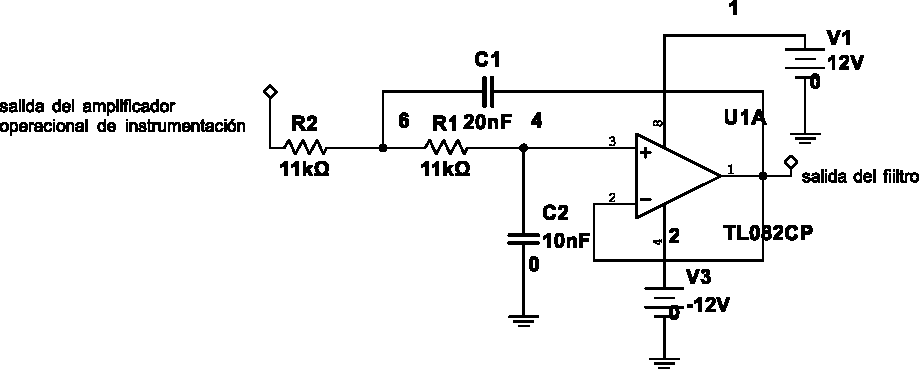
\includegraphics[width=0.6\linewidth]{FiltroEsquematico.pdf}
        \caption{Circuito del filtro anti-aliasing}
        \label{fig:filtroEsquematico}
\end{figure}


\subsection{Buffer}

El buffer tiene como función ser un seguidor de voltaje, es decir, ganancia unitaria.

\begin{figure}[H]
        \centering
        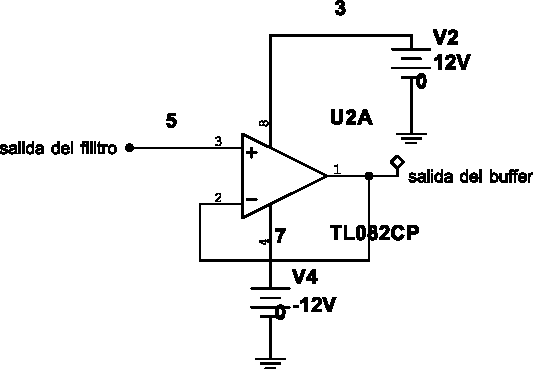
\includegraphics[width=0.35\linewidth]{BufferEsquematico.pdf}
        \caption{Circuito del buffer}
        \label{fig:bufferEsquematico}
\end{figure}

\subsection{ADC}



\section{Simulaciones y análisis}

\subsection{Puente Wheatstone}

\subsection{Filtro anti-alising}

Para simular el filtro anti-aliasing, se utilizó el modelo del TL082. Al ser este filtro tipo pasabajas, se realizó un barrido en corriente alterna para ver el comporatmiento del filtro a distintas frecuencias (de 100~Hz a 10~kHz). El resultado mostró un comportamiento pasabajas esperado, cuyo comportamiento teórico se muestra en la figura~\ref{fig:gananciaFiltro}.

\subsection{Buffer}

La simulación del buffer se realizó utilizando el modelo del TL082, alimentado con una señal de entrada proveniente de una fuente ideal. El resultado mostró que se espera ganancia unitaria en la práctica, con diferencias entre la salida y la entrada nulas o negligibles.

\subsection{ADC}

\section{Resultados Experimentales}
Se llevó a cabo la implementación física del sistema utilizando los circuitos integrados TL082 como amplificadores operacionales y el ADC08.
Se midieron las señales de salida de cada etapa.

\begin{figure}[H]
  \centering
  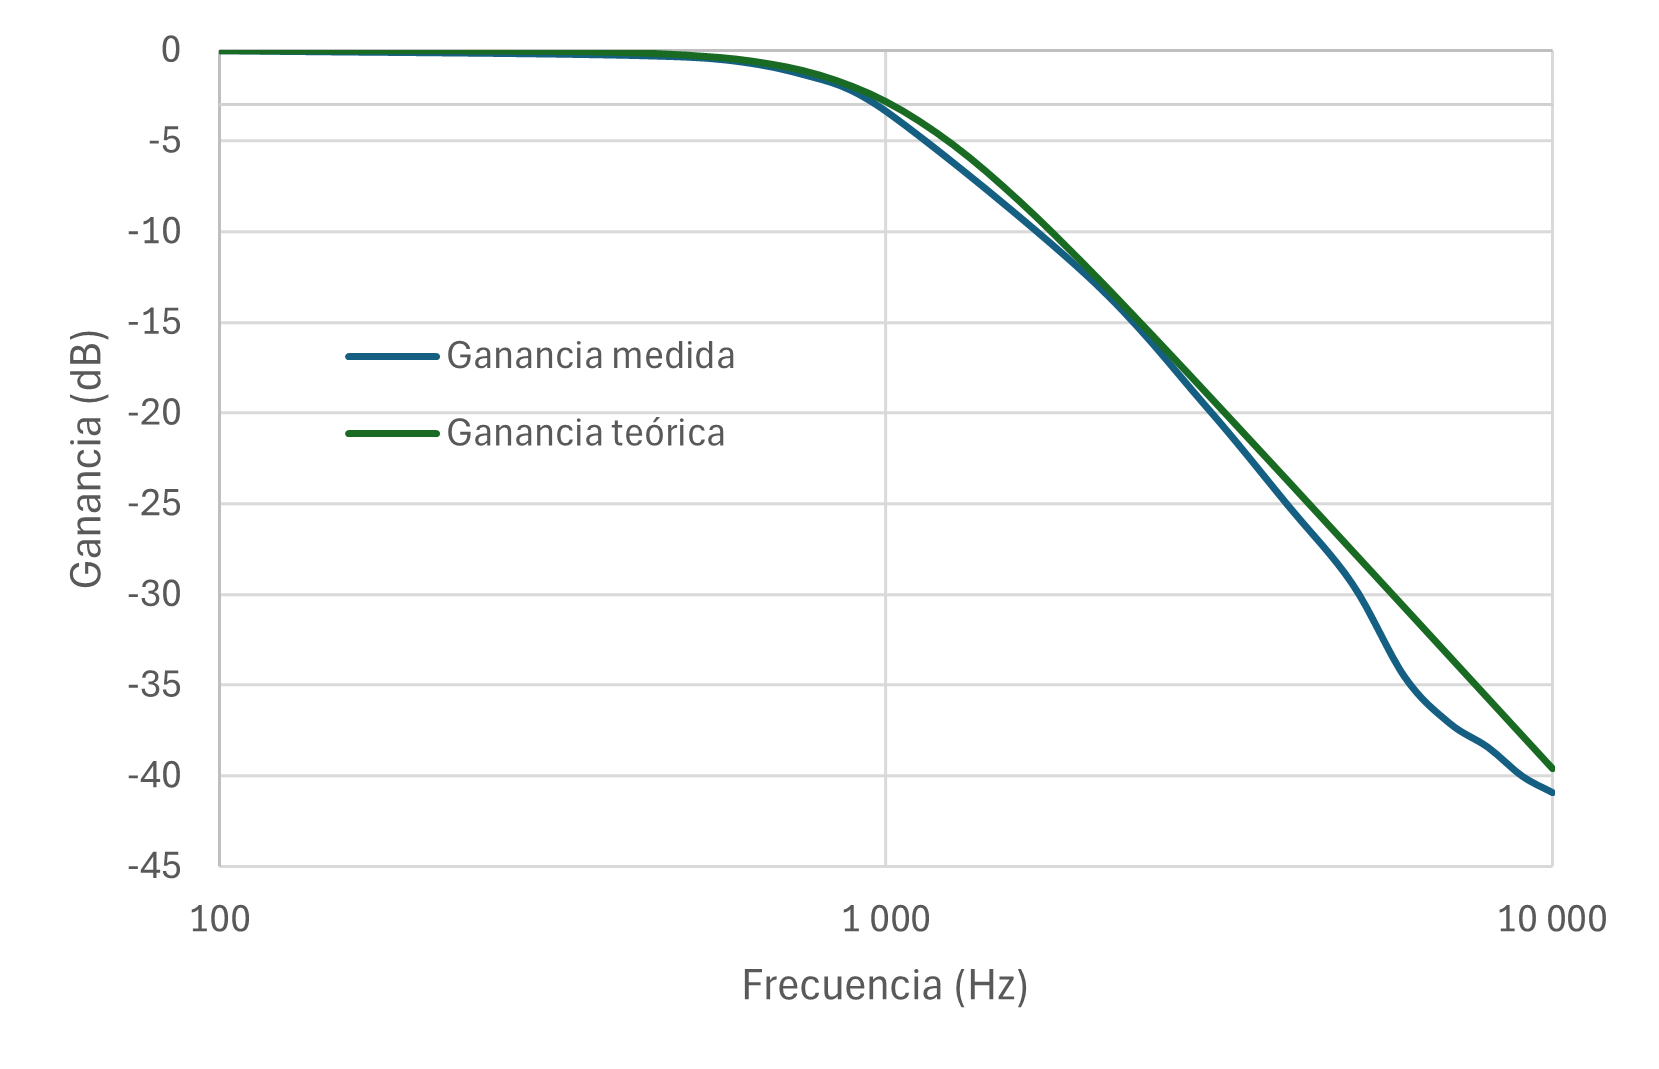
\includegraphics[width=0.6\linewidth]{fig/GananciaFiltro.png} 
  \caption{Ganancia teórica del filtro anti-aliasing y medición de la ganancia}
  \label{fig:gananciaFiltro}
\end{figure}





%%%%%%%%%%%%%%%%%%%%%%%%%%%%%%%%%%%%%%%%%%%%%%%%%%%%%%%%%%%%%%%%%%%%%%%%%%%%%%%%%%%%
%%%%%%%%%%%%%%%%%%%%%%%%%%%%%%%%%%%%%%%%%%%%%%%%%%%%%%%%%%%%%%%%%%%%%%%%%%%%%%%%%%%%
\section{Conclusiones}


%%%%%%%%%%%%%%%%%%%%%%%%%%%%%%%%%%%%%%%%%%%%%%%%%%%%%%%%%%%%%%%%%%%%%%%%%%%%%%%%%%%%
%%%%%%%%%%%%%%%%%%%%%%%%%%%%%%%%%%%%%%%%%%%%%%%%%%%%%%%%%%%%%%%%%%%%%%%%%%%%%%%%%%%%
%\appendices





%%%%%%%%%%%%%%%%%%%%%%%%%%%%%%%%%%%%%%%%%%%%%%%%%%%%%%%%%%%%%%%%%%%%%%%%%%%%%%%%%%%%
%%%%%%%%%%%%%%%%%%%%%%%%%%%%%%%%%%%%%%%%%%%%%%%%%%%%%%%%%%%%%%%%%%%%%%%%%%%%%%%%%%%%

\printbibliography

\vfill

\end{document}






